%% =======================================================
%% Actividad 4: Estadística descriptiva - resumen numérico y gráfico
%%
%% Compilar desde actividades/: ./compilar.sh act04
%% Las figuras de img/ se generan con: python act04.py
%% =======================================================

%% ---- CONFIGURACIÓN ------------------------

\documentclass[11pt,letterpaper]{article}

\usepackage[indice]{tecnm}
\usepackage[T1]{fontenc}
\usepackage{amsmath}
\usepackage{xcolor}
\usepackage[most]{tcolorbox} % Carga tcolorbox con soporte para listings y saltos de página
\tcbuselibrary{listings, skins, breakable}
\setlength{\emergencystretch}{3em} % Evita líneas desbordadas por palabras en \texttt

% Paleta de colores (estilo GitHub Light / VS Code)
\definecolor{codebg}{HTML}{F8F9FA}       % Fondo del código
\definecolor{codehead}{HTML}{E9ECEF}     % Fondo de la barra de título
\definecolor{codeborder}{HTML}{CED4DA}   % Borde de la tarjeta
\definecolor{codetitle}{HTML}{212529}    % Texto del título
\definecolor{codekw}{HTML}{0550AE}       % Palabras clave (import, def, for...)
\definecolor{codefunc}{HTML}{8250DF}     % Funciones y métodos (describe, groupby...)
\definecolor{codestr}{HTML}{0A3069}      % Strings
\definecolor{codecomm}{HTML}{6E7781}     % Comentarios
\definecolor{codenum}{HTML}{8C959F}      % Números de línea
\definecolor{codeid}{HTML}{24292F}       % Texto general

% Configuración base de listings
\lstdefinestyle{pythonestilo}{
  language=Python,
  basicstyle=\ttfamily\footnotesize\color{codeid},
  keywordstyle=\color{codekw}\bfseries,
  keywordstyle=[2]\color{codefunc}, % Estilo secundario para métodos de datos
  stringstyle=\color{teal!80!black},
  commentstyle=\color{codecomm}\itshape,
  morekeywords={as, True, False, None, with, yield, lambda},
  morekeywords=[2]{describe, groupby, value_counts, print, len, sum, sorted, DataFrame, mean, median, mode, multimode, var, std, sqrt, percentile, quantile, Counter, load_iris, load_dataset, hist, boxplot, barplot, heatmap, scatter, axvline, corr, mannwhitneyu, skew, isna, dropna, count},
  numbers=left,
  numberstyle=\tiny\ttfamily\color{codenum},
  stepnumber=1,
  numbersep=10pt,
  showstringspaces=false,
  morestring=[b]{"""},
  tabsize=4,
  breaklines=true,
  breakatwhitespace=true,
  columns=flexible,
  keepspaces=true,
  literate=
    {á}{{\'a}}1 {é}{{\'e}}1 {í}{{\'i}}1 {ó}{{\'o}}1 {ú}{{\'u}}1
    {Á}{{\'A}}1 {É}{{\'E}}1 {Í}{{\'I}}1 {Ó}{{\'O}}1 {Ú}{{\'U}}1
    {ñ}{{\~n}}1 {Ñ}{{\~N}}1 {¿}{{?`}}1 {¡}{{!`}}1
}

% Definición del entorno personalizado \begin{codigo}{Título}{etiqueta}
% \newtcblisting[auto counter, number within=section]{codigo}[2][]{
\newtcblisting[auto counter]{codigo}[2][]{
  listing only,
  breakable,                    % Permite que el bloque se divida si pasa de página
  enhanced,
  colback=codebg,
  colframe=codeborder,
  colbacktitle=codehead,
  coltitle=codetitle,
  fonttitle=\bfseries\small\sffamily,
  boxrule=0.6pt,
  arc=4pt,                      % Bordes redondeados
  left=20pt,                    % Espacio izquierdo para los números de línea
  right=8pt,
  top=6pt,
  bottom=6pt,
  toptitle=4pt,
  bottomtitle=4pt,
  before skip=12pt,
  after skip=12pt,
  listing options={style=pythonestilo},
  title={Código \thetcbcounter: #2},
  #1
}

% Paleta para salida de consola (estilo terminal limpia)
\definecolor{termbg}{HTML}{212529}      % Fondo oscuro tipo terminal
\definecolor{termhead}{HTML}{343A40}    % Barra superior
\definecolor{termtext}{HTML}{F8F9FA}    % Texto claro de alta legibilidad
\definecolor{termborder}{HTML}{495057}  % Borde

% Entorno \begin{consola}[label=out:iris]{Título}
\newtcblisting[auto counter]{consola}[2][]{
  listing only,
  breakable,
  colback=termbg,
  colframe=termborder,
  colbacktitle=termhead,
  coltitle=termtext,
  colupper=termtext,
  fonttitle=\bfseries\small\sffamily,
  boxrule=0.6pt,
  arc=4pt,
  left=8pt,
  right=8pt,
  top=6pt,
  bottom=6pt,
  toptitle=4pt,
  bottomtitle=4pt,
  before skip=12pt,
  after skip=12pt,
  listing options={
    basicstyle=\ttfamily\scriptsize\color{termtext}, % \scriptsize evita que las tablas de Pandas se partan de línea
    breaklines=true,
    columns=fixed,        % Mantiene alineadas las columnas de Pandas
    keepspaces=true,
    showstringspaces=false,
    literate=
      {á}{{\'a}}1 {é}{{\'e}}1 {í}{{\'i}}1 {ó}{{\'o}}1 {ú}{{\'u}}1
      {Á}{{\'A}}1 {É}{{\'E}}1 {Í}{{\'I}}1 {Ó}{{\'O}}1 {Ú}{{\'U}}1
      {ñ}{{\~n}}1 {Ñ}{{\~N}}1
  },
  title={Salida \thetcbcounter: #2},
  #1
}

%% ---- DATOS DE LA MATERIA ------------------------

\materia{Modelos Estadísticos para el Aprendizaje \\ Automático y Ciencia de Datos}
\actividad{Tema 1.3
Estadística Descriptiva: Resumen Numérico y Gráfico \\ Actividad 4 - Cálculo de Medidas Descriptivas y Caso Titanic}

\profesor{Dr. José Ismael Ojeda Campaña}
%\fecha{15 de octubre de 2026}    % opcional; por defecto es la fecha de hoy

\begin{document}
\portada
\indicegeneral

%% ---- CONTENIDO ---------------------------------

\section{Introducción}

La estadística descriptiva resume un conjunto de datos en unos cuantos números y gráficos que describen su centro, su dispersión y su forma. Las medidas de tendencia central (media, mediana y moda) indican cuál es el valor típico de una variable; las medidas de dispersión (varianza, desviación estándar y percentiles) indican qué tanto se alejan los datos de ese valor; y los gráficos, como el histograma y el diagrama de caja, muestran cómo se distribuyen los datos \parencite{tecnm2026_documento_fuente,bruce2020}.

En este documento se resuelven los ejercicios del tema 1.3 en tres partes. Primero, los ocho ejercicios prácticos: seis de cálculo de medidas descriptivas sobre conjuntos pequeños de datos y dos de visualización con el conjunto Iris. Después, el caso de estudio con el conjunto de datos del Titanic, que aplica las mismas medidas a la edad de 891 pasajeros reales. Finalmente, el ejercicio final, que extiende el análisis a la edad, la tarifa y el número de hermanos o cónyuges a bordo, y compara a los pasajeros que sobrevivieron con los que no.

\section{Marco conceptual}

\subsection{Medidas de tendencia central}

Una medida de tendencia central es un valor que representa una entrada típica o central de un conjunto de datos. Las tres más usadas son la media, la mediana y la moda \parencite{tecnm2026_documento_fuente}.

\begin{itemize}
    \item \textbf{Media.} Es la suma de las entradas dividida entre el número de entradas. Para una muestra de $n$ datos:
    \begin{equation}
        \bar{x} = \frac{\sum_{i=1}^{n} x_i}{n}.
    \end{equation}
    \item \textbf{Mediana.} Es el valor que está en medio del conjunto cuando los datos están ordenados. Si el número de datos es impar, es la entrada central; si es par, es la media de las dos entradas centrales \parencite{tecnm2026_documento_fuente}.
    \item \textbf{Moda.} Es la entrada que ocurre con mayor frecuencia. Un conjunto puede tener una moda, más de una (si es bimodal, dos) o ninguna, si ningún valor se repite \parencite{tecnm2026_documento_fuente}.
\end{itemize}

La media usa el valor de todas las observaciones, por lo que es sensible a los valores extremos; la mediana, en cambio, es una medida robusta \parencite{bruce2020}. La relación entre ambas indica la forma de la distribución: en una distribución simétrica coinciden, en una sesgada a la derecha la media es mayor que la mediana, y en una sesgada a la izquierda es menor \parencite{tecnm2026_documento_fuente}.

\subsection{Medidas de dispersión}

La \textbf{varianza} mide cómo se dispersan los datos respecto a la media. Para una muestra se calcula como \parencite{tecnm2026_documento_fuente}:
\begin{equation}
    s^2 = \frac{1}{n - 1} \sum_{i=1}^{n} (x_i - \bar{x})^2.
    \label{eq:varianza}
\end{equation}
Cuando los datos son toda la población, la suma se divide entre $n$ en lugar de $n - 1$. Dividir entre $n - 1$ en una muestra corrige el hecho de que las desviaciones se miden respecto a la media muestral y no respecto a la media real de la población, que es desconocida \parencite{bruce2020}.

La \textbf{desviación estándar} es la raíz cuadrada de la varianza, $s = \sqrt{s^2}$, y expresa la dispersión en las mismas unidades que los datos originales \parencite{tecnm2026_documento_fuente}.

Los \textbf{percentiles} dividen los datos ordenados en 100 partes iguales. El percentil 25 es el primer cuartil ($Q_1$), el percentil 50 es la mediana ($Q_2$) y el percentil 75 es el tercer cuartil ($Q_3$) \parencite{tecnm2026_documento_fuente}. La diferencia $Q_3 - Q_1$ es el rango intercuartílico (RIC), que mide la dispersión del 50\,\% central de los datos \parencite{bruce2020}.

En Python hay que cuidar qué divisor usa cada función. \texttt{np.var()} y \texttt{np.std()} dividen entre $n$ por omisión, salvo que se indique \texttt{ddof=1}; en cambio, los métodos \texttt{.var()} y \texttt{.std()} de \texttt{pandas} dividen entre $n - 1$.

\subsection{Gráficos descriptivos}

Los gráficos son esenciales para visualizar la distribución de los datos y las relaciones entre variables \parencite{tecnm2026_documento_fuente,bruce2020}:

\begin{itemize}
    \item El \textbf{histograma} divide una variable cuantitativa en intervalos y muestra la frecuencia de cada uno.
    \item El \textbf{diagrama de caja} muestra la mediana, los cuartiles $Q_1$ y $Q_3$ (los bordes de la caja), los bigotes, que se extienden hasta los datos que no son atípicos, y los valores atípicos como puntos aislados.
    \item El \textbf{diagrama de dispersión} muestra la relación entre dos variables.
    \item La \textbf{matriz de correlación} muestra la correlación entre cada par de variables numéricas, lo que permite ver de un vistazo cuáles están relacionadas.
    \item El \textbf{gráfico de barras} compara una cantidad entre categorías.
\end{itemize}

\section{Descripción de la actividad}

\textbf{Objetivo:} Calcular e interpretar medidas de tendencia central, de dispersión y percentiles con Python, y aplicarlas, junto con gráficos descriptivos, al análisis de conjuntos de datos reales.

La actividad consta de tres partes \parencite{tecnm2026_documento_fuente}:

\begin{description}
    \item[Ejercicios prácticos.] Calcular la media de 12, 15, 10, 18, 20 (Ejercicio 1); la mediana de 7, 10, 8, 12, 15 (Ejercicio 2); la moda de 5, 7, 5, 10, 5 (Ejercicio 3); la varianza de 5, 7, 9, 6, 10 (Ejercicio 4); la desviación estándar de 15, 17, 19, 13, 20 (Ejercicio 5); y los percentiles 25, 50 y 75 de 8, 14, 10, 12, 18 (Ejercicio 6). Dibujar el histograma (Ejercicio 7) y el diagrama de caja por especie (Ejercicio 8) de la longitud del sépalo del conjunto Iris.
    \item[Caso de estudio Titanic.] Cargar el conjunto de datos (Paso 1); calcular la media y la mediana de la edad y la moda de la clase (Paso 2); la varianza y la desviación estándar de la edad (Paso 3); sus percentiles 25, 50 y 75 (Paso 4); y elaborar el histograma de la edad y su diagrama de caja según la supervivencia (Paso 5).
    \item[Ejercicio final.] Calcular las medidas de tendencia central y de dispersión de la edad, la tarifa y el número de hermanos o cónyuges a bordo; elaborar histogramas, diagramas de caja, un diagrama de dispersión y la matriz de correlación; y analizar qué patrones hay entre los grupos de pasajeros y si existen diferencias significativas entre quienes sobrevivieron y quienes no.
\end{description}

\section{Desarrollo}

Las tres partes se resolvieron en el script \texttt{act04.py}, que usa \texttt{numpy}, \texttt{pandas}, \texttt{scipy}, \texttt{matplotlib} y \texttt{seaborn}. Las figuras se guardan como imágenes PNG en la carpeta \texttt{img/} mediante la función \texttt{guardar()}; cuando el código se ejecuta en un cuaderno, además se muestran en pantalla. El cuaderno interactivo puede consultarse en Google Colab:

\begin{center}
    \url{https://colab.research.google.com/drive/14crrC9vm8dsoMCv0i1_p0fdDNnLD_HOg?usp=sharing}
\end{center}

\subsection{Ejercicios 1 a 6: medidas descriptivas}

Para cada ejercicio se completó el código base del cuaderno de trabajo calculando la medida paso a paso con su fórmula, y se verificó el resultado con la función equivalente de \texttt{numpy} o \texttt{scipy}. En los Ejercicios 4 y 5 se calcularon tanto la versión muestral ($n - 1$) como la poblacional ($n$), para mostrar la diferencia entre ambas. En el Ejercicio 3 se usó \texttt{statistics.multimode()}, que devuelve todas las modas en caso de que haya más de una, como pide el enunciado.

\begin{codigo}[label=cod:ej16]{Ejercicios 1 a 6: media, mediana, moda, varianza, desviación estándar y percentiles}
import math
import os
import statistics
from collections import Counter

import matplotlib

# En Colab o Jupyter no existe __file__; ahí las figuras también se muestran en pantalla
EN_NOTEBOOK = '__file__' not in globals()
if not EN_NOTEBOOK:
    matplotlib.use('Agg')  # Como script, genera las figuras como archivos PNG sin abrir ventanas

import matplotlib.pyplot as plt
import numpy as np
import pandas as pd
import seaborn as sns
from scipy import stats
from sklearn.datasets import load_iris

pd.set_option('display.width', 100)

# Carpeta donde se guardan las figuras que se incluyen en el reporte
BASE = os.getcwd() if EN_NOTEBOOK else os.path.dirname(os.path.abspath(__file__))
CARPETA_IMG = os.path.join(BASE, 'img')
os.makedirs(CARPETA_IMG, exist_ok=True)


def guardar(nombre):
    """Guarda la figura actual en la carpeta img/ y la muestra si se ejecuta en un notebook."""
    plt.tight_layout()
    plt.savefig(os.path.join(CARPETA_IMG, nombre), dpi=150)
    if EN_NOTEBOOK:
        plt.show()
    plt.close()


# Ejercicio 1: cálculo de la media
data = [12, 15, 10, 18, 20]

# Calcular la media
media = sum(data) / len(data)

print("=== Ejercicio 1: media ===")
print(f"Datos: {data}")
print(f"Media con la fórmula (suma / n): {sum(data)} / {len(data)} = {media}")
print(f"Media con np.mean(): {np.mean(data)}")

# Ejercicio 2: cálculo de la mediana
data = [7, 10, 8, 12, 15]

# Calcular la mediana: ordenar y tomar el valor central (n es impar)
ordenados = sorted(data)
mediana = ordenados[len(ordenados) // 2]

print("\n=== Ejercicio 2: mediana ===")
print(f"Datos: {data}")
print(f"Datos ordenados: {ordenados}")
print(f"Mediana (valor central): {mediana}")
print(f"Mediana con np.median(): {np.median(data)}")

# Ejercicio 3: cálculo de la moda
data = [5, 7, 5, 10, 5]

# Calcular la moda: multimode devuelve todas las modas si hay más de una
frecuencias = Counter(data)
modas = statistics.multimode(data)

print("\n=== Ejercicio 3: moda ===")
print(f"Datos: {data}")
print(f"Frecuencias: {dict(frecuencias)}")
print(f"Moda(s): {modas}, aparece {frecuencias[modas[0]]} veces")
moda_scipy = stats.mode(data)
print(f"Moda con stats.mode(): {moda_scipy.mode}, frecuencia {moda_scipy.count}")

# Ejercicio 4: cálculo de la varianza
data = [5, 7, 9, 6, 10]

# Calcular la varianza
media = sum(data) / len(data)
suma_cuadrados = sum((x - media) ** 2 for x in data)
varianza_muestral = suma_cuadrados / (len(data) - 1)
varianza_poblacional = suma_cuadrados / len(data)

print("\n=== Ejercicio 4: varianza ===")
print(f"Datos: {data}")
print(f"Media: {media}")
print(f"Desviaciones al cuadrado: {[round((x - media) ** 2, 2) for x in data]}")
print(f"Suma de cuadrados: {suma_cuadrados:.2f}")
print(f"Varianza muestral (n - 1): {varianza_muestral:.2f}")
print(f"Varianza poblacional (n):  {varianza_poblacional:.2f}")
print(f"np.var(data, ddof=1): {np.var(data, ddof=1):.2f}   np.var(data): {np.var(data):.2f}")

# Ejercicio 5: cálculo de la desviación estándar
data = [15, 17, 19, 13, 20]

# Calcular la desviación estándar (raíz cuadrada de la varianza)
media = sum(data) / len(data)
varianza = sum((x - media) ** 2 for x in data) / (len(data) - 1)
desviacion_estandar = math.sqrt(varianza)

print("\n=== Ejercicio 5: desviación estándar ===")
print(f"Datos: {data}")
print(f"Media: {media}, varianza muestral: {varianza:.2f}")
print(f"Desviación estándar muestral (n - 1): {desviacion_estandar:.4f}")
print(f"Desviación estándar poblacional (n):  {np.std(data):.4f}")

# Ejercicio 6: cálculo de percentiles
data = [8, 14, 10, 12, 18]

# Calcular percentiles
percentiles = np.percentile(data, [25, 50, 75])

print("\n=== Ejercicio 6: percentiles ===")
print(f"Datos: {data}, ordenados: {sorted(data)}")
print(f"Percentiles 25, 50, 75: {percentiles}")
print(f"Rango intercuartílico (Q3 - Q1): {percentiles[2] - percentiles[0]}")
\end{codigo}

\subsection{Ejercicios 7 y 8: visualización del conjunto Iris}

Se ejecutó el código base del cuaderno de trabajo para ambos gráficos. Como extensiones, al histograma se le agregaron la media y la mediana, se dibujó un segundo histograma con un color por especie y se calcularon las estadísticas descriptivas de la variable. Al diagrama de caja se le agregó una tabla con los cuartiles que dibuja cada caja.

\begin{codigo}[label=cod:ej78]{Ejercicios 7 y 8: histograma y diagrama de caja de la longitud del sépalo}
# Cargar el conjunto de datos Iris
iris = load_iris()
df = pd.DataFrame(iris.data, columns=iris.feature_names)
df['species'] = iris.target_names[iris.target]
sepalo = df['sepal length (cm)']

# Código base: histograma para la longitud del sépalo
plt.figure(figsize=(7, 4.5))
plt.hist(sepalo, bins=10, alpha=0.5, color='blue', edgecolor='black')
# Extensión: media y mediana
plt.axvline(sepalo.mean(), color='red', linestyle='--', label=f'Media: {sepalo.mean():.2f}')
plt.axvline(sepalo.median(), color='green', label=f'Mediana: {sepalo.median():.2f}')
plt.title("Histograma de Longitud de Sépalo")
plt.xlabel("Longitud de Sépalo (cm)")
plt.ylabel("Frecuencia")
plt.legend()
guardar('ej7_histograma_iris.png')

# Extensión: histograma por especie para ver de dónde viene la forma general
plt.figure(figsize=(7, 4.5))
for especie, color in zip(iris.target_names, ['tab:blue', 'tab:orange', 'tab:green']):
    plt.hist(sepalo[df['species'] == especie], bins=np.arange(4.2, 8.2, 0.2),
             alpha=0.6, color=color, edgecolor='black', label=especie)
plt.title("Longitud de Sépalo por especie")
plt.xlabel("Longitud de Sépalo (cm)")
plt.ylabel("Frecuencia")
plt.legend()
guardar('ej7_histograma_especies.png')

print("\n=== Ejercicio 7: longitud del sépalo (Iris) ===")
print(sepalo.describe().round(2).to_string())
print(f"Moda(s): {statistics.multimode(sepalo)}")
print(f"Asimetría: {stats.skew(sepalo):.3f}")

# Código base: gráfico de cajas
plt.figure(figsize=(7, 4.5))
sns.boxplot(x=iris.target_names[iris.target], y=df['sepal length (cm)'])
plt.title("Gráfico de Cajas - Longitud del Sépalo")
guardar('ej8_boxplot_iris.png')

# Extensión: los cuartiles que dibuja cada caja
por_especie = sepalo.groupby(df['species']).describe()
por_especie['RIC'] = por_especie['75%'] - por_especie['25%']

print("\n=== Ejercicio 8: longitud del sépalo por especie ===")
print(por_especie[['count', 'mean', 'std', 'min', '25%', '50%', '75%', 'max', 'RIC']].round(2))
\end{codigo}

\subsection{Caso de estudio: Titanic}

El cuaderno de trabajo describe cada paso del caso de estudio y su pregunta, pero no incluye código, por lo que el código de los cinco pasos se escribió a partir de esas descripciones. El conjunto de datos del Titanic se cargó con \texttt{sns.load\_dataset('titanic')}, como indica el cuaderno, y sus primeras filas coinciden con la salida esperada del Paso 1. Contiene 891 pasajeros, pero la edad falta en 177 de ellos. Los métodos de \texttt{pandas} ignoran automáticamente los valores faltantes, por lo que todas las medidas de la edad se calculan sobre los 714 pasajeros con edad registrada. La varianza y la desviación estándar de \texttt{pandas} usan el divisor $n - 1$ de la ecuación~\eqref{eq:varianza}.

\begin{codigo}[label=cod:titanic]{Caso de estudio Titanic: pasos 1 a 5}
# Paso 1: cargar y examinar los datos
titanic = sns.load_dataset('titanic')

print("\n=== Caso Titanic - Paso 1: datos ===")
print(titanic.head())
print(f"\nDimensiones: {titanic.shape}")
print("Valores faltantes por columna:")
print(titanic.isna().sum()[lambda s: s > 0].to_string())

edad = titanic['age']  # pandas ignora los 177 valores faltantes en los cálculos

# Paso 2: medidas de tendencia central
print("\n=== Caso Titanic - Paso 2: tendencia central ===")
print(f"Media de la edad: {edad.mean():.2f} años")
print(f"Mediana de la edad: {edad.median():.2f} años")
print(f"Moda de la clase (pclass): {titanic['pclass'].mode()[0]}")
print(titanic['pclass'].value_counts().sort_index().to_string())

# Paso 3: medidas de dispersión (pandas usa n - 1 por omisión)
print("\n=== Caso Titanic - Paso 3: dispersión ===")
print(f"Varianza de la edad: {edad.var():.2f} años^2")
print(f"Desviación estándar de la edad: {edad.std():.2f} años")

# Paso 4: percentiles
print("\n=== Caso Titanic - Paso 4: percentiles ===")
print(edad.quantile([0.25, 0.50, 0.75]).to_string())

# Paso 5: histograma de la edad y boxplot por supervivencia
plt.figure(figsize=(7, 4.5))
plt.hist(edad.dropna(), bins=30, color='steelblue', edgecolor='black')
plt.axvline(edad.mean(), color='red', linestyle='--', label=f'Media: {edad.mean():.1f}')
plt.axvline(edad.median(), color='green', label=f'Mediana: {edad.median():.1f}')
plt.title('Distribución de la edad de los pasajeros')
plt.xlabel('Edad (años)')
plt.ylabel('Número de pasajeros')
plt.legend()
guardar('titanic_histograma_edad.png')

plt.figure(figsize=(7, 4.5))
sns.boxplot(data=titanic, x='survived', y='age', hue='survived',
            palette=['salmon', 'mediumseagreen'], legend=False)
plt.xticks([0, 1], ['No sobrevivió', 'Sobrevivió'])
plt.title('Edad de los pasajeros según supervivencia')
plt.xlabel('')
plt.ylabel('Edad (años)')
guardar('titanic_boxplot_edad.png')

print("\n=== Caso Titanic - Paso 5: edad por supervivencia ===")
print(titanic.groupby('survived')['age'].describe().round(2))
\end{codigo}

\subsection{Ejercicio final: análisis completo del Titanic}

La función \texttt{medidas()} calcula la media, la mediana, la moda, la varianza y la desviación estándar de una variable. Se aplicó a la edad, la tarifa y el número de hermanos o cónyuges a bordo (\texttt{sibsp}), primero para todos los pasajeros y después por separado para quienes sobrevivieron y quienes no. Se elaboraron los cuatro gráficos que pide el ejercicio: histogramas y diagramas de caja de las tres variables por supervivencia, un diagrama de dispersión de edad contra tarifa y la matriz de correlación de las variables numéricas. En el diagrama de dispersión, la tarifa se dibujó en escala logarítmica, porque su distribución es muy asimétrica.

Como extensiones, para identificar patrones en los grupos de pasajeros se calculó la tasa de supervivencia por sexo y por clase, con su gráfico de barras. Además, para responder si las diferencias entre sobrevivientes y no sobrevivientes son \textit{significativas}, se aplicó la prueba de Mann-Whitney a cada variable. Esta prueba no paramétrica compara si dos grupos independientes provienen de la misma distribución y no requiere que los datos sean normales \parencite{tecnm2026_documento_fuente}, lo que es importante porque la tarifa y \texttt{sibsp} están muy sesgadas. Un valor $p < 0.05$ indica que la diferencia entre los grupos es estadísticamente significativa.

\begin{codigo}[label=cod:final]{Ejercicio final: análisis completo del Titanic}
variables = {'age': 'Edad', 'fare': 'Tarifa', 'sibsp': 'Hermanos/cónyuges'}


def medidas(serie):
    """Medidas de tendencia central y dispersión de una variable."""
    return {'Media': serie.mean(), 'Mediana': serie.median(), 'Moda': serie.mode()[0],
            'Varianza': serie.var(), 'Desv. est.': serie.std(), 'n': serie.count()}


print("\n=== Ejercicio final: medidas de todos los pasajeros ===")
print(pd.DataFrame({nombre: medidas(titanic[col]) for col, nombre in variables.items()})
      .round(2))

print("\n=== Ejercicio final: medidas por supervivencia ===")
for col, nombre in variables.items():
    tabla = pd.DataFrame({etiqueta: medidas(grupo[col]) for etiqueta, grupo in
                          titanic.groupby(titanic['survived'].map({0: 'No sobrevivió',
                                                                   1: 'Sobrevivió'}))})
    print(f"\n{nombre}:")
    print(tabla.round(2))

# Tasa de supervivencia por sexo y por clase
print("\n=== Ejercicio final: tasa de supervivencia por grupo ===")
print((titanic.groupby('sex')['survived'].mean() * 100).round(1).to_string())
print((titanic.groupby('pclass')['survived'].mean() * 100).round(1).to_string())

# Prueba de Mann-Whitney: ¿las distribuciones difieren entre sobrevivientes y no?
print("\n=== Ejercicio final: prueba de Mann-Whitney (sobrevivió vs. no) ===")
for col, nombre in variables.items():
    sobrevivio = titanic.loc[titanic['survived'] == 1, col].dropna()
    no_sobrevivio = titanic.loc[titanic['survived'] == 0, col].dropna()
    resultado = stats.mannwhitneyu(sobrevivio, no_sobrevivio)
    print(f"{nombre:<18} U = {resultado.statistic:>9.1f}   p = {resultado.pvalue:.2g}")

colores = {0: 'salmon', 1: 'mediumseagreen'}
etiquetas = {0: 'No sobrevivió', 1: 'Sobrevivió'}

# Histogramas de las tres variables por supervivencia
fig, axes = plt.subplots(1, 3, figsize=(13, 4))
rangos = {'age': np.arange(0, 85, 5), 'fare': np.arange(0, 525, 25), 'sibsp': np.arange(-0.5, 9)}
for ax, (col, nombre) in zip(axes, variables.items()):
    for s in (0, 1):
        ax.hist(titanic.loc[titanic['survived'] == s, col].dropna(), bins=rangos[col],
                alpha=0.6, color=colores[s], edgecolor='black', label=etiquetas[s])
    ax.set_title(nombre)
    ax.set_ylabel('Número de pasajeros')
axes[0].legend()
guardar('final_histogramas.png')

# Diagramas de caja de las tres variables por supervivencia
fig, axes = plt.subplots(1, 3, figsize=(13, 4))
for ax, (col, nombre) in zip(axes, variables.items()):
    sns.boxplot(data=titanic, x='survived', y=col, hue='survived', ax=ax,
                palette=list(colores.values()), legend=False)
    ax.set_xticks([0, 1], list(etiquetas.values()))
    ax.set_xlabel('')
    ax.set_ylabel(nombre)
guardar('final_boxplots.png')

# Diagrama de dispersión de edad vs. tarifa por supervivencia
plt.figure(figsize=(8, 5))
for s in (0, 1):
    grupo = titanic[titanic['survived'] == s]
    plt.scatter(grupo['age'], grupo['fare'], color=colores[s], alpha=0.6,
                edgecolor='gray', linewidth=0.3, label=etiquetas[s])
plt.yscale('symlog', linthresh=10)  # La tarifa es muy asimétrica
plt.title('Edad vs. tarifa según supervivencia')
plt.xlabel('Edad (años)')
plt.ylabel('Tarifa (escala logarítmica)')
plt.legend()
guardar('final_dispersion.png')

# Matriz de correlación de las variables numéricas
numericas = titanic[['survived', 'pclass', 'age', 'sibsp', 'parch', 'fare']]
correlacion = numericas.corr()
plt.figure(figsize=(7, 5.5))
sns.heatmap(correlacion, annot=True, fmt='.2f', cmap='coolwarm', vmin=-1, vmax=1,
            square=True)
plt.title('Matriz de correlación')
guardar('final_correlacion.png')

# Tasa de supervivencia por sexo y clase
plt.figure(figsize=(7, 4.5))
sns.barplot(data=titanic, x='pclass', y='survived', hue='sex', errorbar=None,
            palette=['steelblue', 'orchid'])
plt.title('Tasa de supervivencia por clase y sexo')
plt.xlabel('Clase')
plt.ylabel('Proporción que sobrevivió')
guardar('final_supervivencia.png')

print("\n=== Ejercicio final: correlación con survived ===")
print(correlacion['survived'].drop('survived').round(3).to_string())

print(f"\nFiguras guardadas en {os.path.basename(CARPETA_IMG)}/")
\end{codigo}

\section{Resultados}

\subsection{Ejercicios 1 a 6: medidas descriptivas}

\begin{consola}[label=out:ej16]{Ejecución de \texttt{act04.py}: Ejercicios 1 a 6}
=== Ejercicio 1: media ===
Datos: [12, 15, 10, 18, 20]
Media con la fórmula (suma / n): 75 / 5 = 15.0
Media con np.mean(): 15.0

=== Ejercicio 2: mediana ===
Datos: [7, 10, 8, 12, 15]
Datos ordenados: [7, 8, 10, 12, 15]
Mediana (valor central): 10
Mediana con np.median(): 10.0

=== Ejercicio 3: moda ===
Datos: [5, 7, 5, 10, 5]
Frecuencias: {5: 3, 7: 1, 10: 1}
Moda(s): [5], aparece 3 veces
Moda con stats.mode(): 5, frecuencia 3

=== Ejercicio 4: varianza ===
Datos: [5, 7, 9, 6, 10]
Media: 7.4
Desviaciones al cuadrado: [5.76, 0.16, 2.56, 1.96, 6.76]
Suma de cuadrados: 17.20
Varianza muestral (n - 1): 4.30
Varianza poblacional (n):  3.44
np.var(data, ddof=1): 4.30   np.var(data): 3.44

=== Ejercicio 5: desviación estándar ===
Datos: [15, 17, 19, 13, 20]
Media: 16.8, varianza muestral: 8.20
Desviación estándar muestral (n - 1): 2.8636
Desviación estándar poblacional (n):  2.5612

=== Ejercicio 6: percentiles ===
Datos: [8, 14, 10, 12, 18], ordenados: [8, 10, 12, 14, 18]
Percentiles 25, 50, 75: [10. 12. 14.]
Rango intercuartílico (Q3 - Q1): 4.0
\end{consola}

La Tabla~\ref{tab:ejercicios} resume las respuestas a las preguntas de los seis ejercicios.

\begin{table}[htbp]
\centering
\caption{Respuestas de los Ejercicios 1 a 6.}
\label{tab:ejercicios}
\begin{tabular}{clll}
\hline
\textbf{Ej.} & \textbf{Datos} & \textbf{Medida} & \textbf{Resultado} \\
\hline
1 & 12, 15, 10, 18, 20 & Media & 15 \\
2 & 7, 10, 8, 12, 15 & Mediana & 10 \\
3 & 5, 7, 5, 10, 5 & Moda & 5 (aparece 3 veces) \\
4 & 5, 7, 9, 6, 10 & Varianza & 4.30 (muestral); 3.44 (poblacional) \\
5 & 15, 17, 19, 13, 20 & Desviación estándar & 2.86 (muestral); 2.56 (poblacional) \\
6 & 8, 14, 10, 12, 18 & Percentiles 25, 50, 75 & $Q_1 = 10$, $Q_2 = 12$, $Q_3 = 14$ \\
\hline
\end{tabular}
\end{table}

\begin{enumerate}
    \item \textbf{¿Cuál es el valor de la media?} La media es $\bar{x} = 75 / 5 = \mathbf{15}$.
    \item \textbf{¿Cuál es el valor de la mediana?} Al ordenar los datos (7, 8, \textbf{10}, 12, 15), el valor central es \textbf{10}. Como hay cinco datos, la mediana es la tercera entrada.
    \item \textbf{¿Cuál es la moda y cuántas veces aparece?} La moda es \textbf{5}, que aparece \textbf{3 veces}. Es la única moda, porque 7 y 10 aparecen una sola vez; \texttt{multimode()} lo confirma al devolver una lista con un solo valor.
    \item \textbf{¿Cuál es el valor de la varianza?} La media es 7.4 y la suma de las desviaciones al cuadrado es 17.2. Tratando los datos como una muestra, como en la ecuación~\eqref{eq:varianza}, la varianza es $17.2 / 4 = \mathbf{4.30}$. Si se trataran como una población completa, sería $17.2 / 5 = 3.44$, que es el valor que devuelve \texttt{np.var()} por omisión.
    \item \textbf{¿Cuál es el valor de la desviación estándar?} La varianza muestral es 8.2, por lo que la desviación estándar es $\sqrt{8.2} \approx \mathbf{2.86}$. La versión poblacional, que devuelve \texttt{np.std()} por omisión, es 2.56. Es decir, los datos se alejan en promedio unas 2.9 unidades de su media de 16.8.
    \item \textbf{¿Cuáles son los percentiles 25, 50 y 75?} Con los datos ordenados (8, 10, 12, 14, 18), \texttt{np.percentile()} da $Q_1 = \mathbf{10}$, $Q_2 = \mathbf{12}$ y $Q_3 = \mathbf{14}$. El percentil 50 coincide con la mediana, y el rango intercuartílico es $14 - 10 = 4$.
\end{enumerate}

La diferencia entre las versiones muestral y poblacional de los Ejercicios 4 y 5 es importante en la práctica: con solo cinco datos, dividir entre 4 o entre 5 cambia la varianza en un 25\,\%. Como estos datos representan una muestra, el valor adecuado es el muestral, y conviene indicar \texttt{ddof=1} explícitamente al usar \texttt{numpy}.

\subsection{Ejercicio 7: histograma de la longitud del sépalo}

\begin{figure}[htbp]
\centering
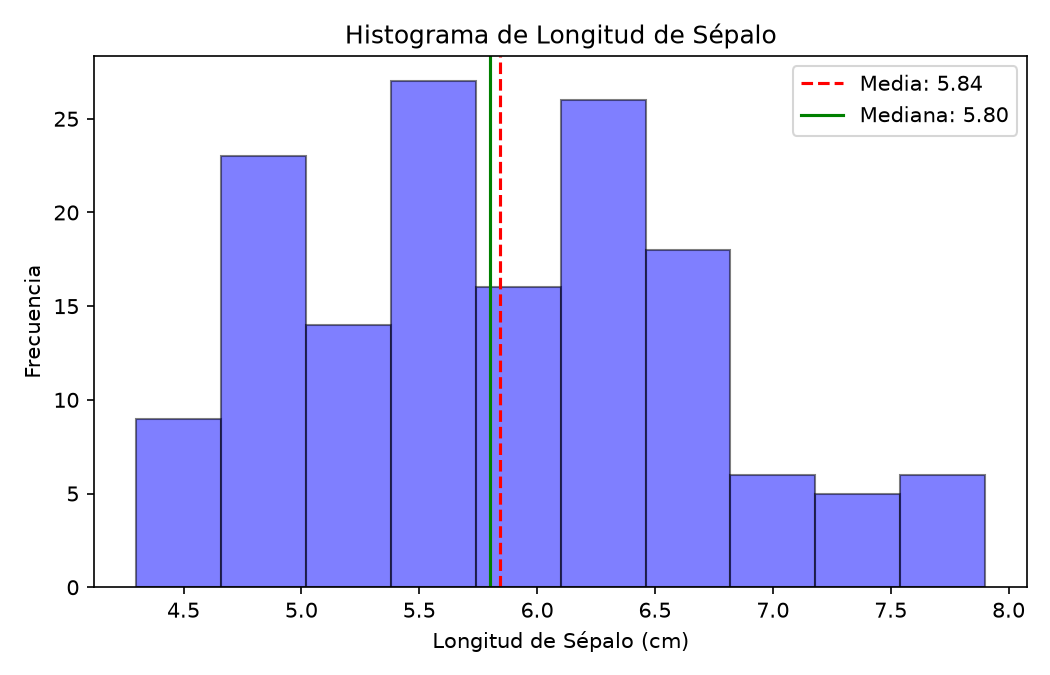
\includegraphics[width=0.49\textwidth]{img/ej7_histograma_iris.png}
\hfill
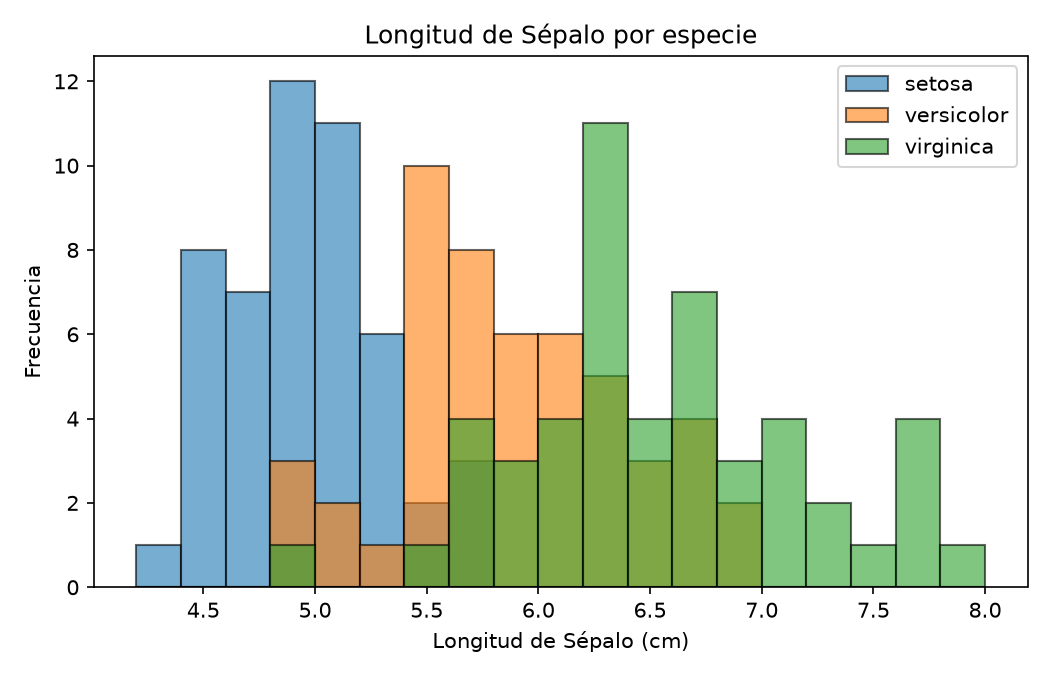
\includegraphics[width=0.49\textwidth]{img/ej7_histograma_especies.png}
\caption{Izquierda: histograma de la longitud del sépalo de las 150 flores del conjunto Iris. Derecha: el mismo histograma separado por especie.}
\label{fig:hist_iris}
\end{figure}

\begin{consola}[label=out:ej7]{Ejecución de \texttt{act04.py}: Ejercicio 7}
=== Ejercicio 7: longitud del sépalo (Iris) ===
count    150.00
mean       5.84
std        0.83
min        4.30
25%        5.10
50%        5.80
75%        6.40
max        7.90
Moda(s): [5.0]
Asimetría: 0.312
\end{consola}

\textbf{¿Qué información proporciona el histograma sobre la distribución de la longitud del sépalo?}

\begin{itemize}
    \item \textbf{Centro y rango.} La longitud del sépalo va de 4.3 a 7.9\,cm, con la mayoría de las flores entre 5 y 6.5\,cm. La media (5.84\,cm) y la mediana (5.80\,cm) casi coinciden, y la mitad central de las flores está entre 5.1 y 6.4\,cm.
    \item \textbf{Forma.} La distribución es casi simétrica, con una ligera cola hacia la derecha (asimetría de 0.31): hay pocas flores con sépalos mayores a 7\,cm.
    \item \textbf{Mezcla de grupos.} El histograma no tiene un solo pico bien definido, sino una forma irregular con varios máximos locales. El histograma por especie (Figura~\ref{fig:hist_iris}, derecha) explica por qué: la distribución general es la mezcla de tres distribuciones centradas en valores distintos. \textit{Setosa} concentra los sépalos cortos, \textit{virginica} los largos y \textit{versicolor} queda en medio, traslapándose con ambas.
\end{itemize}

\subsection{Ejercicio 8: diagrama de caja por especie}

\begin{figure}[htbp]
\centering
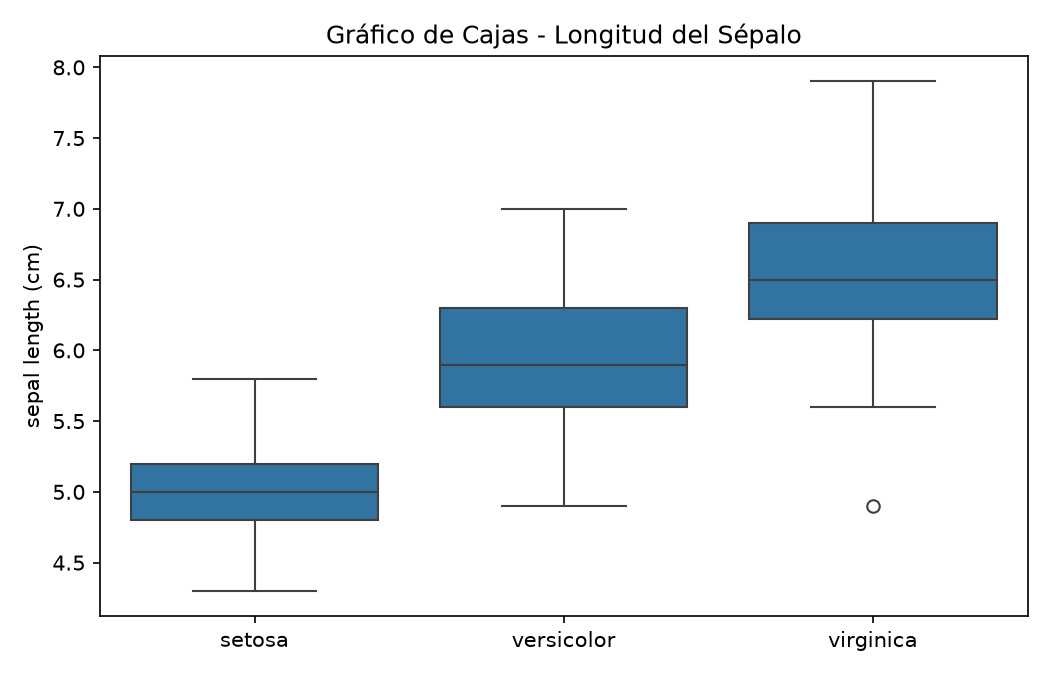
\includegraphics[width=0.68\textwidth]{img/ej8_boxplot_iris.png}
\caption{Diagrama de caja de la longitud del sépalo por especie del conjunto Iris.}
\label{fig:box_iris}
\end{figure}

\begin{consola}[label=out:ej8]{Ejecución de \texttt{act04.py}: Ejercicio 8}
=== Ejercicio 8: longitud del sépalo por especie ===
            count  mean   std  min   25%  50%  75%  max   RIC
species
setosa       50.0  5.01  0.35  4.3  4.80  5.0  5.2  5.8  0.40
versicolor   50.0  5.94  0.52  4.9  5.60  5.9  6.3  7.0  0.70
virginica    50.0  6.59  0.64  4.9  6.22  6.5  6.9  7.9  0.68
\end{consola}

\textbf{¿Qué se puede observar acerca de la distribución de la longitud del sépalo para las diferentes especies?}

\begin{itemize}
    \item \textbf{Centro.} Las medianas crecen de \textit{setosa} (5.0\,cm) a \textit{versicolor} (5.9\,cm) y a \textit{virginica} (6.5\,cm). Las cajas de \textit{setosa} y \textit{virginica} no se traslapan: el 75\,\% de las \textit{setosa} mide 5.2\,cm o menos, mientras que el 75\,\% de las \textit{virginica} mide 6.22\,cm o más.
    \item \textbf{Dispersión.} \textit{Setosa} es la especie más homogénea, con un RIC de solo 0.40\,cm y una desviación estándar de 0.35\,cm. \textit{Versicolor} y \textit{virginica} son más variables, con RIC cercanos a 0.7\,cm.
    \item \textbf{Valores atípicos.} \textit{Virginica} tiene un valor atípico de 4.9\,cm, una flor con un sépalo inusualmente corto para su especie.
    \item \textbf{Utilidad para clasificar.} La longitud del sépalo distingue bien a \textit{setosa} de \textit{virginica}, pero \textit{versicolor} se traslapa con ambas, por lo que esta variable sola no basta para clasificar las tres especies.
\end{itemize}

\subsection{Caso de estudio: Titanic}

\begin{consola}[label=out:titanic]{Ejecución de \texttt{act04.py}: caso de estudio Titanic}
=== Caso Titanic - Paso 1: datos ===
   survived  pclass     sex   age  ...  deck  embark_town  alive  alone
0         0       3    male  22.0  ...   NaN  Southampton     no  False
1         1       1  female  38.0  ...     C    Cherbourg    yes  False
2         1       3  female  26.0  ...   NaN  Southampton    yes   True
3         1       1  female  35.0  ...     C  Southampton    yes  False
4         0       3    male  35.0  ...   NaN  Southampton     no   True

[5 rows x 15 columns]

Dimensiones: (891, 15)
Valores faltantes por columna:
age            177
embarked         2
deck           688
embark_town      2

=== Caso Titanic - Paso 2: tendencia central ===
Media de la edad: 29.70 años
Mediana de la edad: 28.00 años
Moda de la clase (pclass): 3
pclass
1    216
2    184
3    491

=== Caso Titanic - Paso 3: dispersión ===
Varianza de la edad: 211.02 años^2
Desviación estándar de la edad: 14.53 años

=== Caso Titanic - Paso 4: percentiles ===
0.25    20.125
0.50    28.000
0.75    38.000

=== Caso Titanic - Paso 5: edad por supervivencia ===
          count   mean    std   min   25%   50%   75%   max
survived
0         424.0  30.63  14.17  1.00  21.0  28.0  39.0  74.0
1         290.0  28.34  14.95  0.42  19.0  28.0  36.0  80.0
\end{consola}

Las respuestas a las preguntas de los pasos 2 a 4 son:

\begin{itemize}
    \item \textbf{Media de la edad:} 29.70 años.
    \item \textbf{Mediana de la edad:} 28 años. La media es algo mayor que la mediana, lo que anticipa un ligero sesgo a la derecha.
    \item \textbf{Moda de la clase:} la tercera clase, con 491 de los 891 pasajeros (55\,\%).
    \item \textbf{Varianza de la edad:} 211.02\,años$^2$. Al estar en unidades al cuadrado, es difícil de interpretar directamente.
    \item \textbf{Desviación estándar de la edad:} 14.53 años; las edades se alejan, en promedio, unos 14.5 años de la media.
    \item \textbf{Percentiles 25, 50 y 75 de la edad:} 20.125, 28 y 38 años. La mitad central de los pasajeros tenía entre 20 y 38 años.
\end{itemize}

Todas estas medidas se calcularon sobre los 714 pasajeros con edad registrada; la edad falta en 177 pasajeros, casi el 20\,\% del total.

\begin{figure}[htbp]
\centering
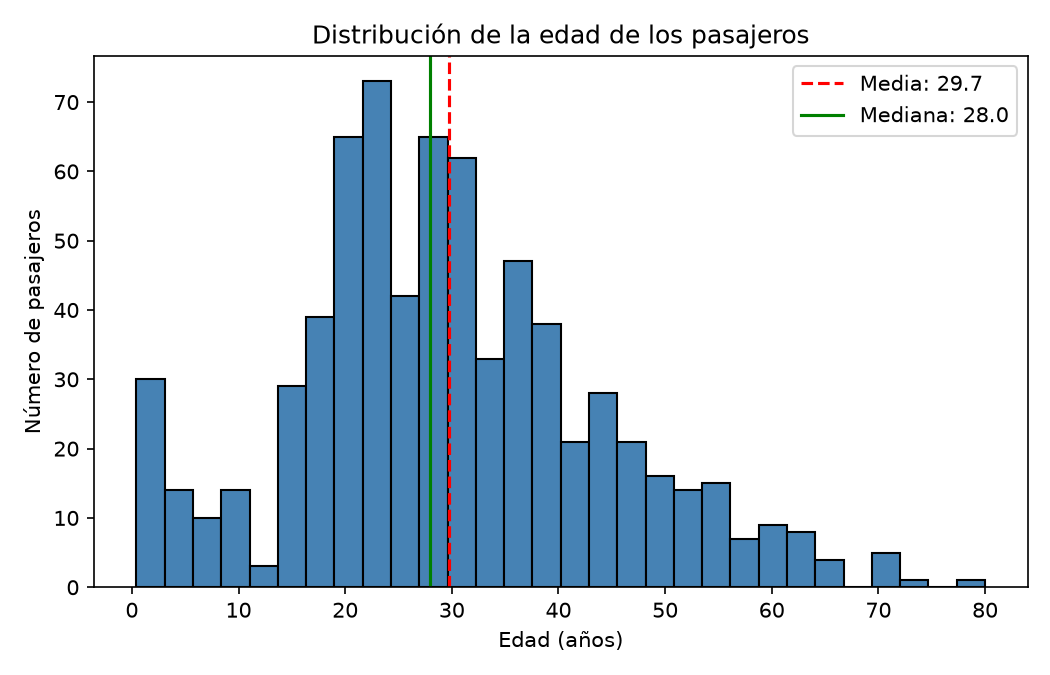
\includegraphics[width=0.49\textwidth]{img/titanic_histograma_edad.png}
\hfill
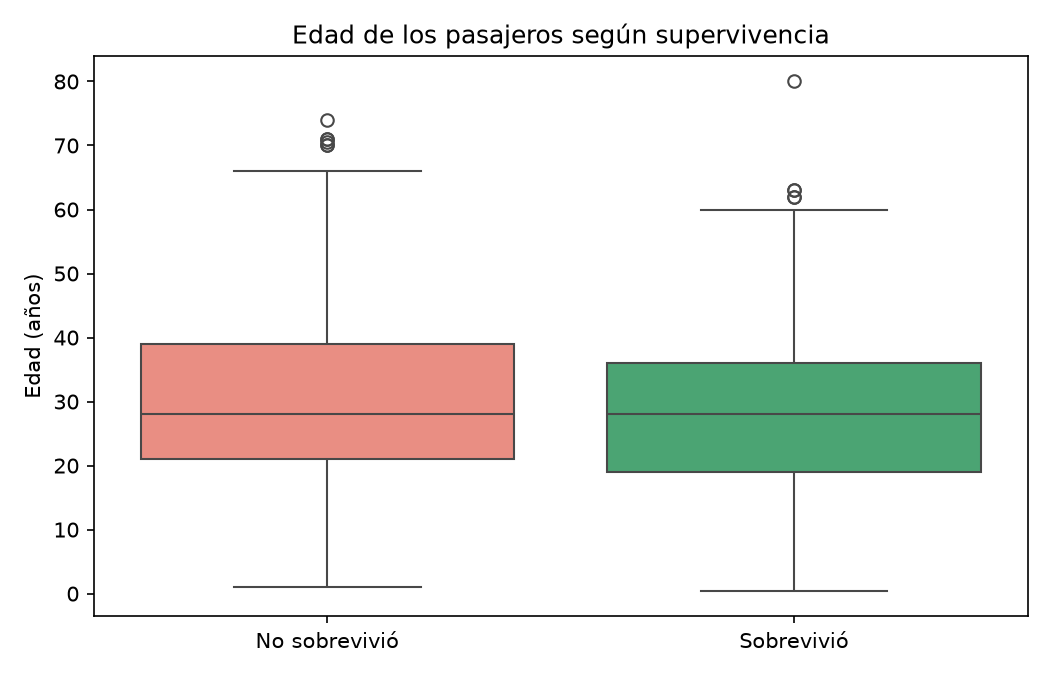
\includegraphics[width=0.49\textwidth]{img/titanic_boxplot_edad.png}
\caption{Izquierda: histograma de la edad de los pasajeros del Titanic. Derecha: diagrama de caja de la edad según la supervivencia.}
\label{fig:titanic_edad}
\end{figure}

\textbf{¿Qué información se obtiene del histograma sobre la distribución de la edad?} La mayoría de los pasajeros eran adultos jóvenes: el pico está entre los 20 y los 30 años. La distribución tiene un sesgo a la derecha, con una cola de pasajeros mayores que llega hasta los 80 años, lo que explica que la media (29.7) sea mayor que la mediana (28). También hay un grupo pequeño pero visible de niños menores de 5 años, que forman un segundo pico al inicio de la distribución.

\textbf{¿Qué se puede observar sobre la edad de los pasajeros que sobrevivieron y los que no?} Las dos cajas son muy parecidas: ambos grupos tienen la misma mediana (28 años) y rangos intercuartílicos similares. Los sobrevivientes son ligeramente más jóvenes, con una media de 28.34 años contra 30.63, y su caja empieza más abajo ($Q_1$ de 19 años contra 21). Esto refleja la mayor supervivencia de los niños. Aun así, la diferencia es pequeña: la edad, por sí sola, no distingue claramente a quienes sobrevivieron.

\subsection{Ejercicio final: análisis completo del Titanic}

\begin{consola}[label=out:final]{Ejecución de \texttt{act04.py}: ejercicio final}
=== Ejercicio final: medidas de todos los pasajeros ===
              Edad   Tarifa  Hermanos/cónyuges
Media        29.70    32.20               0.52
Mediana      28.00    14.45               0.00
Moda         24.00     8.05               0.00
Varianza    211.02  2469.44               1.22
Desv. est.   14.53    49.69               1.10
n           714.00   891.00             891.00

=== Ejercicio final: medidas por supervivencia ===

Edad:
            No sobrevivió  Sobrevivió
Media               30.63       28.34
Mediana             28.00       28.00
Moda                21.00       24.00
Varianza           200.85      223.53
Desv. est.          14.17       14.95
n                  424.00      290.00

Tarifa:
            No sobrevivió  Sobrevivió
Media               22.12       48.40
Mediana             10.50       26.00
Moda                 8.05       13.00
Varianza           985.22     4435.16
Desv. est.          31.39       66.60
n                  549.00      342.00

Hermanos/cónyuges:
            No sobrevivió  Sobrevivió
Media                0.55        0.47
Mediana              0.00        0.00
Moda                 0.00        0.00
Varianza             1.66        0.50
Desv. est.           1.29        0.71
n                  549.00      342.00

=== Ejercicio final: tasa de supervivencia por grupo ===
sex
female    74.2
male      18.9
pclass
1    63.0
2    47.3
3    24.2

=== Ejercicio final: prueba de Mann-Whitney (sobrevivió vs. no) ===
Edad               U =   57682.0   p = 0.16
Tarifa             U =  129951.5   p = 4.6e-22
Hermanos/cónyuges  U =  101983.0   p = 0.008

=== Ejercicio final: correlación con survived ===
pclass   -0.338
age      -0.077
sibsp    -0.035
parch     0.082
fare      0.257

Figuras guardadas en img/
\end{consola}

\begin{figure}[htbp]
\centering
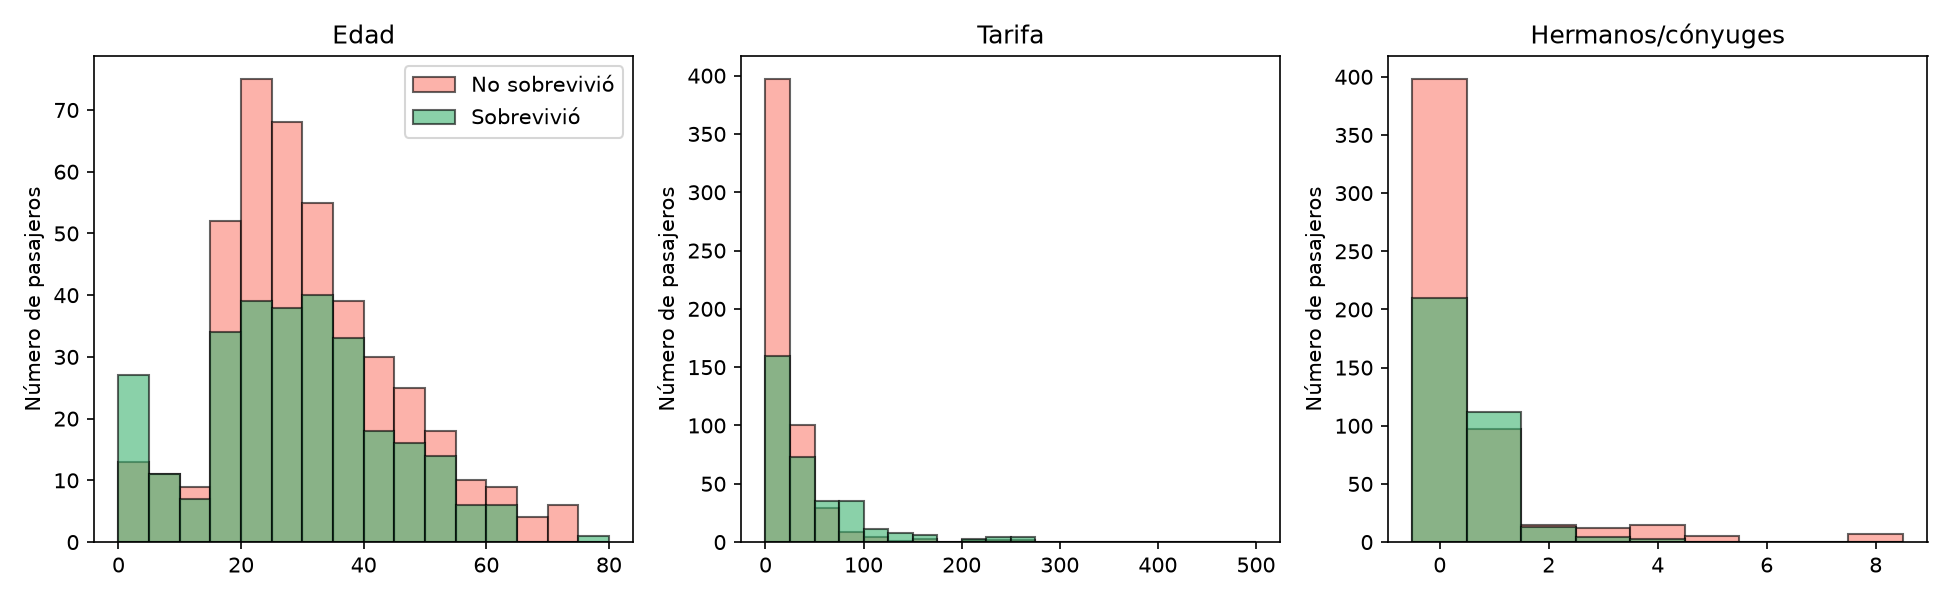
\includegraphics[width=\textwidth]{img/final_histogramas.png}
\caption{Histogramas de la edad, la tarifa y el número de hermanos o cónyuges a bordo, según la supervivencia.}
\label{fig:final_hist}
\end{figure}

\begin{figure}[htbp]
\centering
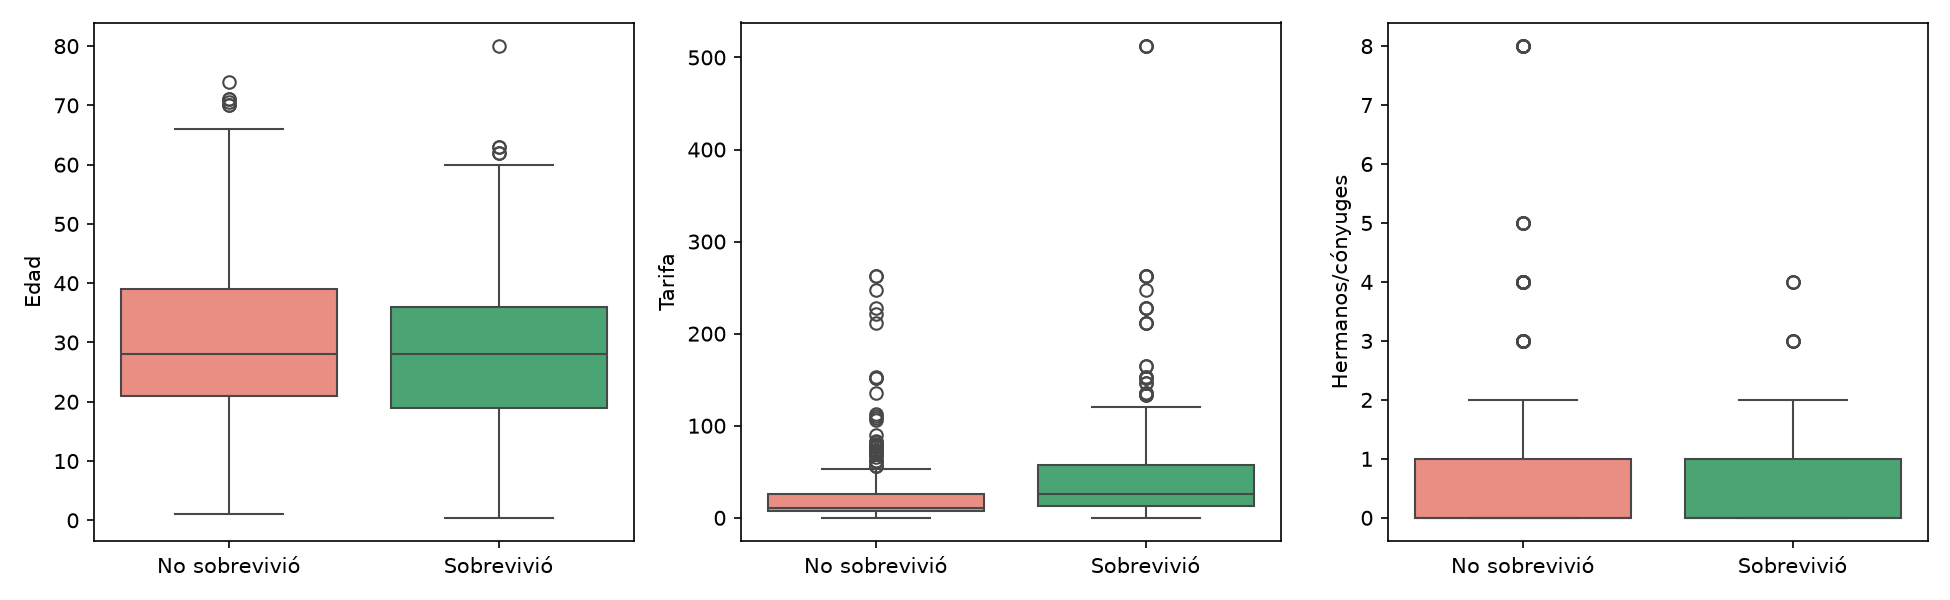
\includegraphics[width=\textwidth]{img/final_boxplots.png}
\caption{Diagramas de caja de la edad, la tarifa y el número de hermanos o cónyuges a bordo, según la supervivencia.}
\label{fig:final_box}
\end{figure}

\begin{figure}[htbp]
\centering
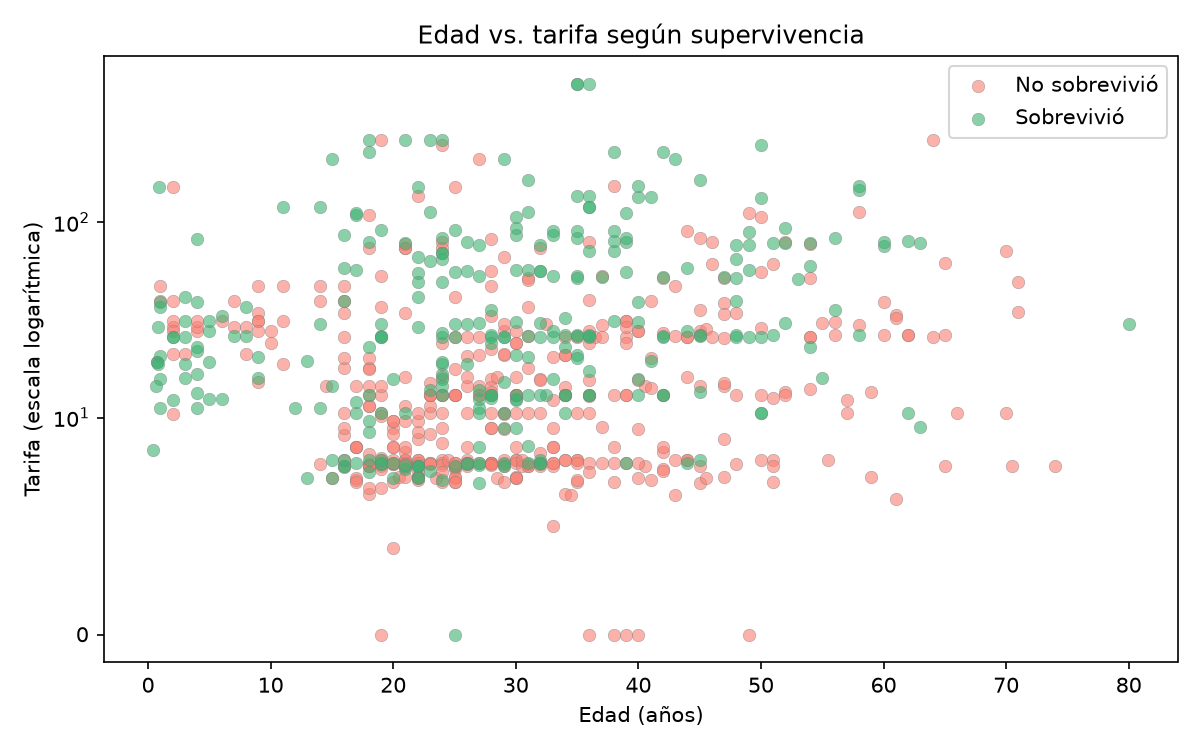
\includegraphics[width=0.75\textwidth]{img/final_dispersion.png}
\caption{Diagrama de dispersión de la edad contra la tarifa (en escala logarítmica), según la supervivencia.}
\label{fig:final_disp}
\end{figure}

\begin{figure}[htbp]
\centering
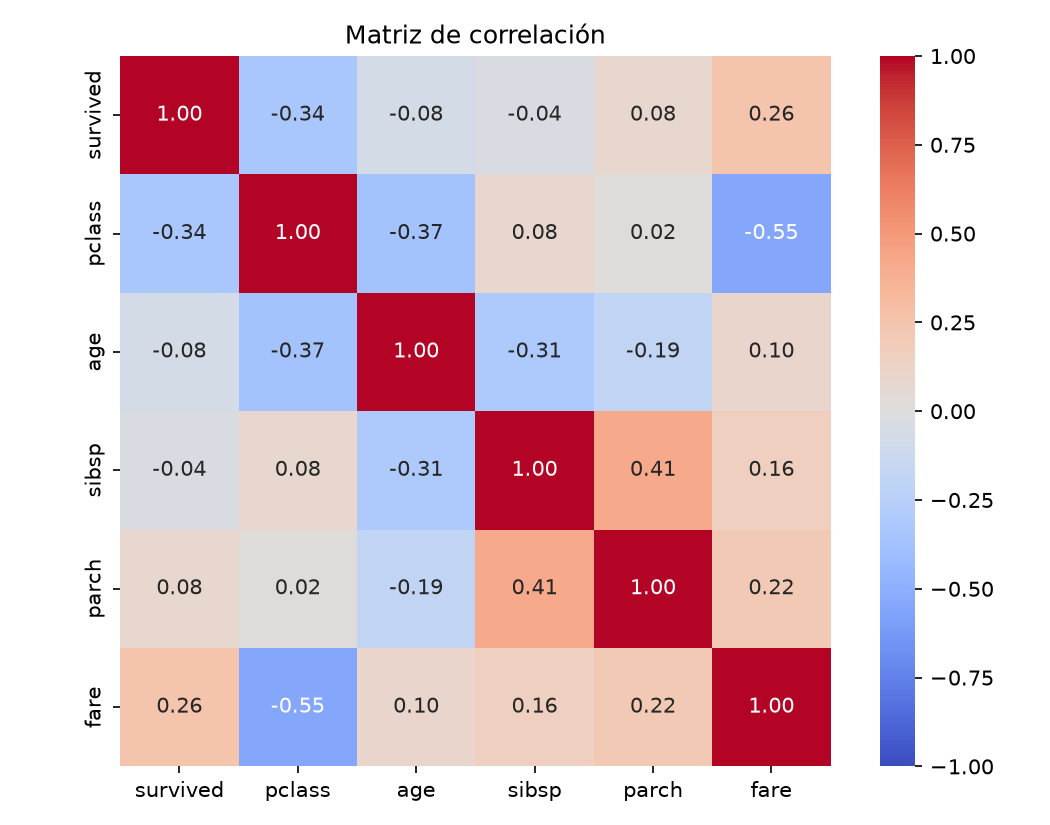
\includegraphics[width=0.49\textwidth]{img/final_correlacion.png}
\hfill
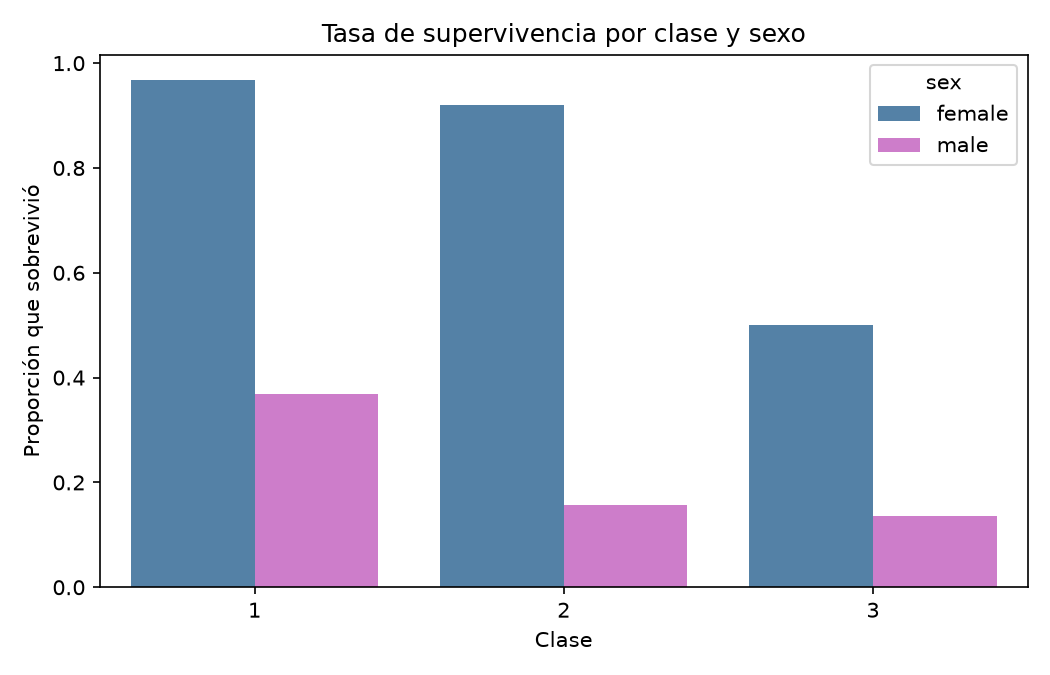
\includegraphics[width=0.49\textwidth]{img/final_supervivencia.png}
\caption{Izquierda: matriz de correlación de las variables numéricas. Derecha: tasa de supervivencia por clase y sexo.}
\label{fig:final_corr}
\end{figure}

\textbf{Medidas de las tres variables.} Las tres variables tienen formas muy distintas, como muestra la Figura~\ref{fig:final_hist}:

\begin{itemize}
    \item La \textbf{edad} es casi simétrica: su media (29.70) y su mediana (28) están cerca, y la moda es de 24 años.
    \item La \textbf{tarifa} está muy sesgada a la derecha. La mayoría pagó poco (la moda es de 8.05 y la mediana de 14.45), pero unas cuantas tarifas muy altas, de hasta 512, elevan la media a 32.20 y la desviación estándar a 49.69, mayor que la propia media.
    \item El \textbf{número de hermanos o cónyuges} es una variable discreta y concentrada en 0: tanto la mediana como la moda son 0, es decir, la mayoría viajaba sin hermanos ni cónyuge. Unos pocos pasajeros de familias numerosas, con hasta 8 hermanos, hacen que la media sea de 0.52.
\end{itemize}

\textbf{¿Qué patrones se observan en los diferentes grupos de pasajeros?}

\begin{itemize}
    \item \textbf{Sexo.} Es el factor más marcado: sobrevivió el 74.2\,\% de las mujeres y solo el 18.9\,\% de los hombres, lo que refleja el criterio de evacuación de ``mujeres y niños primero''.
    \item \textbf{Clase.} La supervivencia cae de forma clara con la clase: 63.0\,\% en primera, 47.3\,\% en segunda y 24.2\,\% en tercera. La Figura~\ref{fig:final_corr} (derecha) muestra que ambos efectos se combinan: casi todas las mujeres de primera y segunda clase sobrevivieron (96.8\,\% y 92.1\,\%), mientras que en tercera clase sobrevivió solo la mitad de ellas, y en los hombres de segunda y tercera clase la supervivencia no llegó al 16\,\%.
    \item \textbf{Tarifa.} Los sobrevivientes pagaron tarifas mucho mayores: su mediana es de 26 contra 10.50 de los que no sobrevivieron. En el diagrama de dispersión (Figura~\ref{fig:final_disp}), los puntos verdes predominan en la parte alta, con tarifas mayores a 50, y los rojos se concentran en las tarifas bajas. La tarifa está muy relacionada con la clase (correlación de $-0.55$ con \texttt{pclass}: a mejor clase, mayor tarifa), por lo que su efecto refleja en buena parte el de la clase.
    \item \textbf{Edad.} El diagrama de dispersión no muestra una separación clara por edad, salvo en los niños: la mayoría de los pasajeros menores de 10 años sobrevivió.
    \item \textbf{Familia.} Viajar con un hermano o cónyuge se asocia con mayor supervivencia: el 32.7\,\% de los sobrevivientes tenía exactamente uno, contra el 17.7\,\% de los no sobrevivientes. En cambio, todos los pasajeros con 5 u 8 hermanos murieron.
\end{itemize}

\textbf{¿Hay diferencias significativas entre quienes sobrevivieron y quienes no?} Según la prueba de Mann-Whitney:

\begin{itemize}
    \item \textbf{Tarifa:} la diferencia es altamente significativa ($p = 4.6 \times 10^{-22}$). Es la variable numérica que más distingue a los dos grupos, lo que coincide con su correlación de 0.26 con la supervivencia.
    \item \textbf{Hermanos o cónyuges:} la diferencia también es significativa ($p = 0.008$), aunque ambas medianas son 0. La prueba detecta que la distribución completa es distinta: entre los sobrevivientes es más común tener un hermano o cónyuge, y entre los no sobrevivientes son más comunes tanto viajar solo como pertenecer a una familia numerosa. Como el efecto no es monótono, la correlación lineal con la supervivencia es casi nula ($-0.035$).
    \item \textbf{Edad:} la diferencia no es significativa ($p = 0.16$). Aunque los sobrevivientes son en promedio dos años más jóvenes, esa diferencia puede deberse al azar.
\end{itemize}

En la matriz de correlación, la variable más relacionada con la supervivencia es la clase ($-0.34$: a mayor número de clase, menor supervivencia), seguida de la tarifa (0.26). El sexo no aparece en la matriz porque es una variable categórica, pero el gráfico de barras muestra que es el factor con mayor efecto.

\section{Conclusiones}

Los ejercicios con datos pequeños permitieron calcular cada medida a mano y comprobarla con las funciones de Python. Esto hizo visible un detalle práctico importante: \texttt{numpy} calcula por omisión la varianza y la desviación estándar poblacionales (dividiendo entre $n$), mientras que \texttt{pandas} y la fórmula muestral dividen entre $n - 1$. Con cinco datos, la diferencia es del 25\,\% en la varianza, por lo que siempre conviene saber qué versión se está calculando.

Los ejemplos con datos reales mostraron que las medidas numéricas y los gráficos se complementan. En el conjunto Iris, la media y la mediana indicaban una distribución casi simétrica, pero solo el histograma por especie y el diagrama de caja revelaron que la longitud del sépalo es una mezcla de tres grupos. En el Titanic, la comparación entre media y mediana anticipó el sesgo de la tarifa, cuya media duplica la mediana, y la presencia de 177 edades faltantes obligó a revisar sobre qué datos se calculaba cada medida.

Finalmente, el análisis del Titanic mostró cómo la estadística descriptiva permite identificar los factores asociados a un resultado. El sexo y la clase fueron los factores más marcados en la supervivencia, y la tarifa fue la variable numérica con la diferencia más significativa entre sobrevivientes y no sobrevivientes. La edad, en cambio, solo mostró un efecto claro en los niños. Agregar una prueba estadística a la comparación descriptiva permitió distinguir las diferencias reales, como la de la tarifa, de las que pueden deberse al azar, como la de la edad.

\referencias

\end{document}
